% !TeX root = skripta-konstitutivni-vztahy.tex
% !TeX lastmodified = 2018-12-04

\subsection{Podmínka plasticity Mohr-Coulomb}\label{sec:mohr-coulomb}
Představuje rozšíření Trescovy podmínky na materiály s~různou mezí kluzu v~tahu a~tlaku.
Její redukované napětí je dáno rovnicí
\begin{multline}
	\sigma_\text{red}^\text{MC}
	= \frac{m+1}{2} \max\Big[
	\left|\sigma_\text{I} - \sigma_\text{II}\right| + K \left(\sigma_\text{I} + \sigma_\text{II}\right);
	\left|\sigma_\text{I} - \sigma_\text{III}\right| + K \left(\sigma_\text{I} + \sigma_\text{III}\right);\\
	\left|\sigma_\text{II} - \sigma_\text{III}\right| + K \left(\sigma_\text{II} + \sigma_\text{III}\right)
	\Big],
\end{multline}
kde
\begin{equation*}
	m = \frac{R_e^\text{tlak}}{R_e^\text{tah}}
	\qquad\text{a}\qquad
	K = \frac{m-1}{m+1}
\end{equation*}
a~v~Haighově prostoru hlavních napětí představuje pravidelný šestiboký jehlan.
\begin{figure}[H]
	\centering
	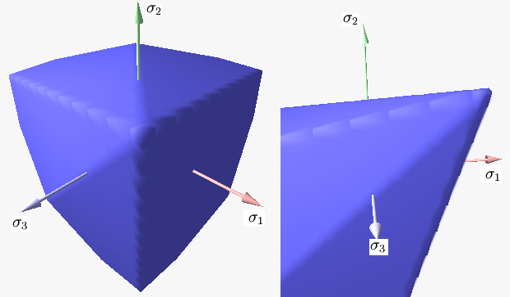
\includegraphics[width=0.5\linewidth]{mohr-coulomb}
	\caption{Podmínka plasticity Mohr-Coulomb v~Heighově prostoru}
	\label{fig:mohr-coulomb}
\end{figure}

Pozor! Pro výpočet součinitele bezpečnosti je třeba použít mez kluzu v~tlaku!
\begin{equation}
	k = \frac{R_e^\text{tlak}}{\sigma_\text{red}^\text{MC}}
\end{equation}

Pro $m=1$ dostaneme standardní tvar Trescovy podmínky.
